\documentclass[hide notes,intlimits]{beamer}

\mode<presentation>
{
  \usetheme[footline]{UAFshadealert}
  \setbeamercovered{transparent}
}

% frames are 128 millimeters by 96 millimeters

% load packages
\usepackage[english]{babel}
\usepackage[latin1]{inputenc}
\usepackage[T1]{fontenc}
\usepackage{amsmath,amssymb,wasysym}
\usepackage{lmodern}

\usepackage{tikz}
\usetikzlibrary{shapes,arrows,shadows}

\usepackage{empheq}
\usepackage{color}
\usepackage{animate}

\graphicspath{{figures/}}

% Some useful commands (from MPL)
\newcommand{\s}[1]{\ensuremath{\,\text{#1}}}
\newcommand{\unit}[1]{\ensuremath{\,\text{#1}}}

\definecolor{dark red}{HTML}{E41A1C}
\definecolor{dark green}{HTML}{4DAF4A}
\definecolor{dark violet}{HTML}{984EA3}
\definecolor{dark blue}{HTML}{084594}
\definecolor{dark orange}{HTML}{FF7F00}
\definecolor{light blue}{HTML}{377EB8}
\definecolor{light red}{HTML}{FB9A99}
\definecolor{light violet}{HTML}{CAB2D6}

\setbeamercolor{boxed}{fg=black,bg=uaf yellow}


\newenvironment{transbox}{%
  
\begin{tikzpicture}
    \node[drop shadow,rounded corners,text width=\textwidth,fill=white, fill opacity=0.6,text opacity=1] \bgroup
  }{
    \egroup;\end{tikzpicture}} 

\newenvironment{transbox-tight}{%
  \begin{tikzpicture}
    \node[drop shadow,rounded corners,fill=uaf yellow, fill opacity=0.75,text opacity=1] \bgroup
  }{
    \egroup;\end{tikzpicture}} 


% title page
\title[Better subglacial hydrology into PISM]{Better subglacial hydrology into \\ the Parallel Ice Sheet Model}
\subtitle{definitely a work in progress}

\author[Bueler \and van Pelt]{Ed Bueler\inst{*} and Ward van Pelt\inst{\dagger}}
\institute{\inst{*} University of Alaska Fairbanks \and %
           \inst{\dagger} IMAU, Utrecht, Netherlands}

\date{IGS June 2012}


\begin{document}

\setbeamertemplate{background canvas}
{
  % empty
}

% insert titlepage
\begin{frame}
  \titlepage
\end{frame}


\newcommand{\scream}[1]{\alert{\textbf{#1}}}

\begin{frame}
  \frametitle{PISM = Parallel Ice Sheet Model}

  \begin{center}
      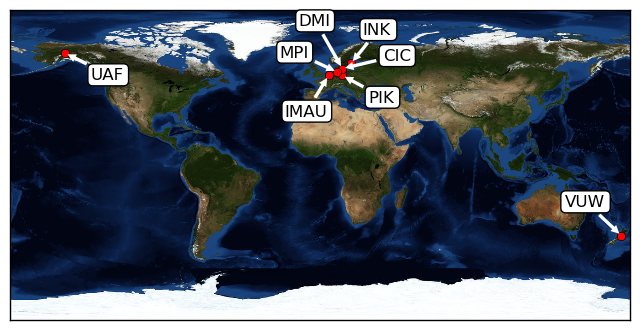
\includegraphics[width=80mm]{figs/pism-users-map}
  \end{center}

\vspace{-2mm}
  \begin{itemize}
  \item \alert{\large\texttt{www.pism-docs.org}}  and  \url{help@pism-docs.org}
  \item runs on laptops to supercomputers
  \item documented releases once a year
  \item \emph{User's Manual} with real modeling examples including Greenland Ice Sheet, Ross Ice Shelf, and St\"orglaciaren
  
  \bigskip
  \scriptsize
  \item[$\circ$] supported by the NASA Modeling, Analysis and Prediction (grant NNX09AJ38G)
  \item[$\circ$] jointly developed by UAF and the Potsdam Institute for Climate Impact Research
  \end{itemize}
\end{frame}


\newcommand{\whytitle}{why we need better subglacial hydrology}

\begin{frame}
  \frametitle{\whytitle}
  \framesubtitle{motivation 1}

\vspace{-6mm}
\begin{center}
  we are \scream{NOT} conserving mass (of liquid water)
\end{center}

\vspace{-5mm}
\begin{columns}
\begin{column}{0.5\textwidth}
  \begin{itemize}
    \item current basal hydrology in PISM has an independent ``can'' of porous till at each subglacial location %$\longrightarrow$
      \begin{itemize}
        \item[$\ast$] the can receives basal melt
        \item[$\ast$] ``overflows'' at 2m of water \dots overflow lost
        \item[$\ast$] \dots but it provides till yield stress in reasonable way
        \item[$\ast$] suitable for Siple coast ice streams (Tulaczyk et al 2000) %$\longrightarrow$
      \end{itemize}
    \item missing:
    
      \begin{center} \emph{lateral transport of water} \end{center}
  \end{itemize}
\end{column}
\begin{column}{0.5\textwidth}
\begin{center}
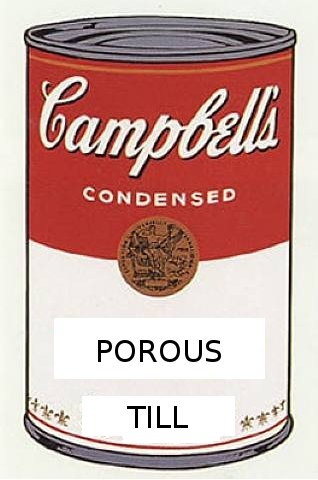
\includegraphics[height=0.3\textheight]{figs/till-warhol-soup}

%\vspace{1mm}

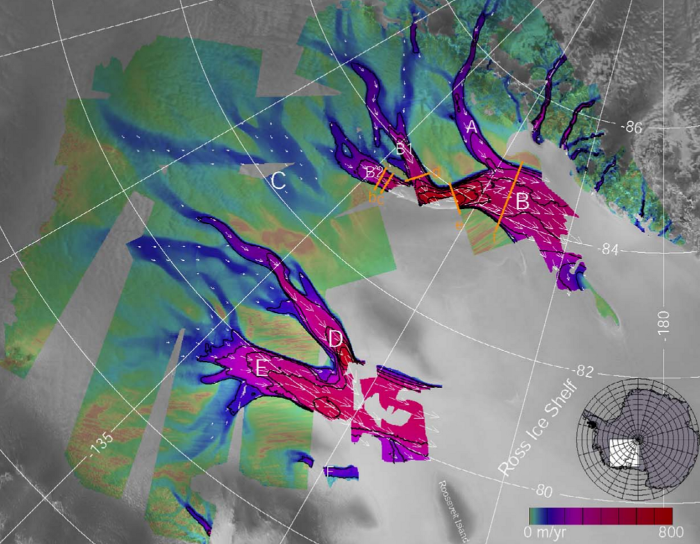
\includegraphics[height=0.45\textheight]{figs/siple}
\end{center}
\end{column}
\end{columns}
\end{frame}


\begin{frame}
  \frametitle{\whytitle}
  \framesubtitle{motivation 2}

\vspace{-6mm}
\begin{center}
  we \scream{ARE} conserving energy (better than before)
\end{center}
  
\vspace{-2mm}
  \begin{itemize}
    \item better energy conservation using enthalpy
    \item new basal melt rate equation
    %\item \emph{lots of water comes from dissipating gravitational potential energy, and some from geothermal energy}
  \end{itemize}

  \begin{center}
    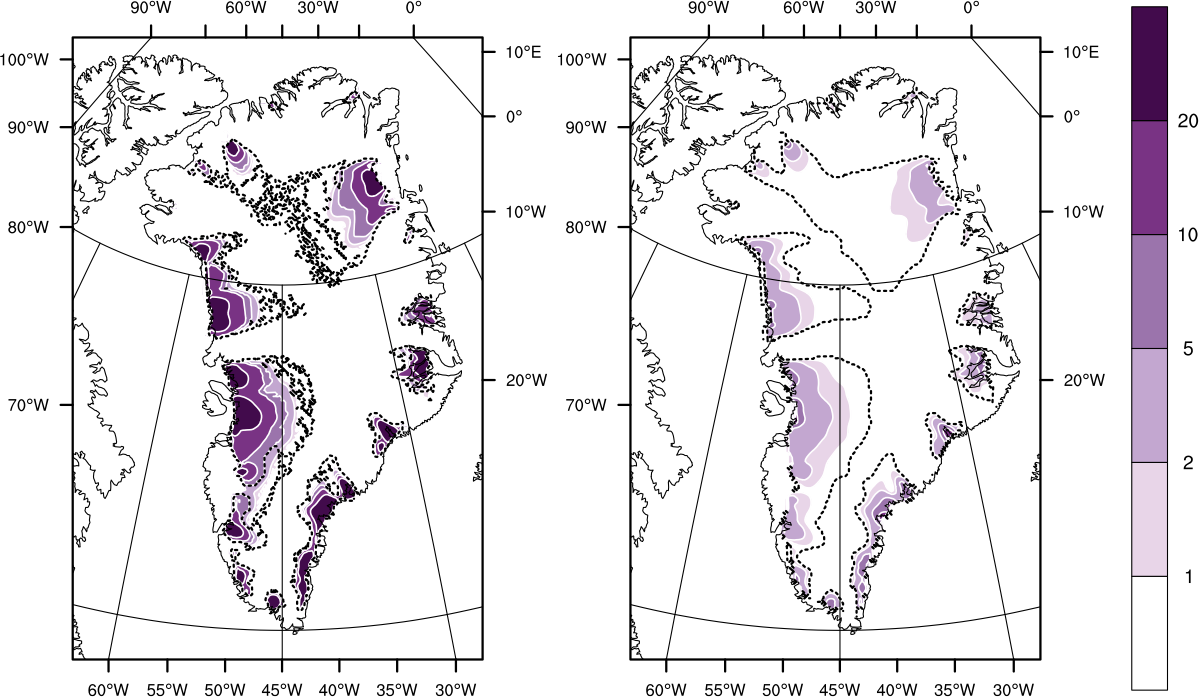
\includegraphics[height=0.6\textheight]{figs/enthalpy-model-crop}
    
    \medskip
    \scriptsize \textbf{left}: basal melt rate using \underline{enthalpy} \qquad \textbf{right}: basal melt rate using \underline{temperature}

    \tiny (from Aschwanden et al (2012) \emph{An enthalpy formulation for glaciers and ice sheets}, J. Glaciol.)
  \end{center}
\end{frame}


\begin{frame}
  \frametitle{existing uses of PISM subglacial hydrology}

\begin{columns}
\begin{column}{0.5\textwidth}
\begin{center}
\textbf{typical purpose:} model the locations of all Antarctic ice streams without inversion

\vspace{11mm}

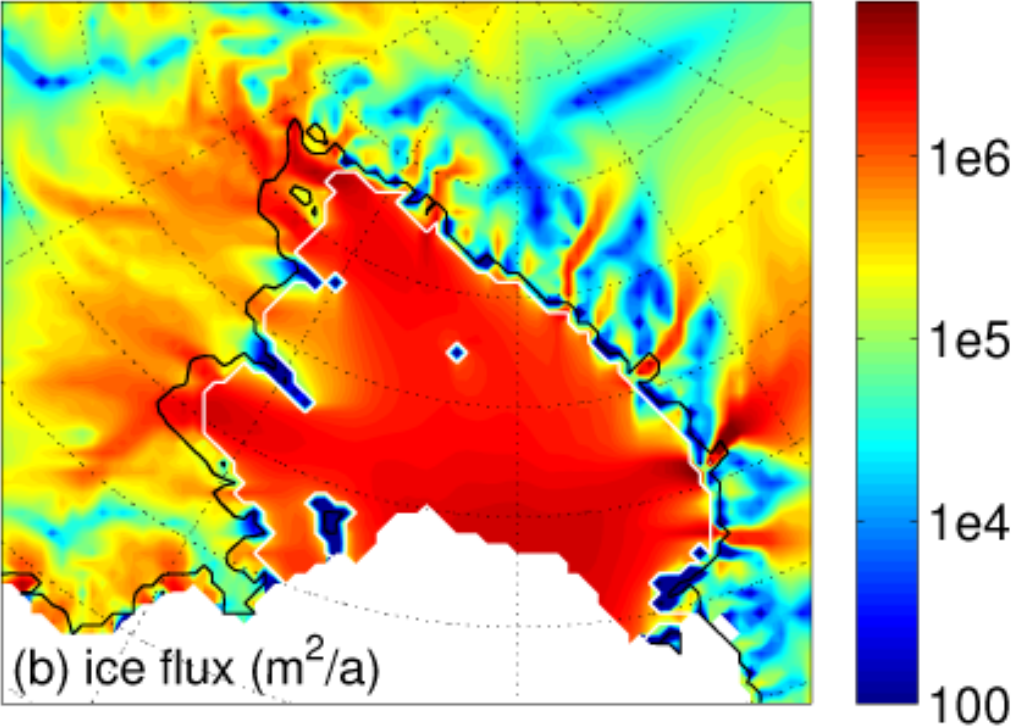
\includegraphics[width=0.9\textwidth]{figs/martin-fig12}

\vspace{5mm}

\medskip
\scriptsize (Martin et al., 2011, \emph{The Cryosphere})
\end{center}
\end{column}
\begin{column}{0.5\textwidth}
\begin{center}
\textbf{less typical:} study sliding/surging cyclicity in PISM

\bigskip
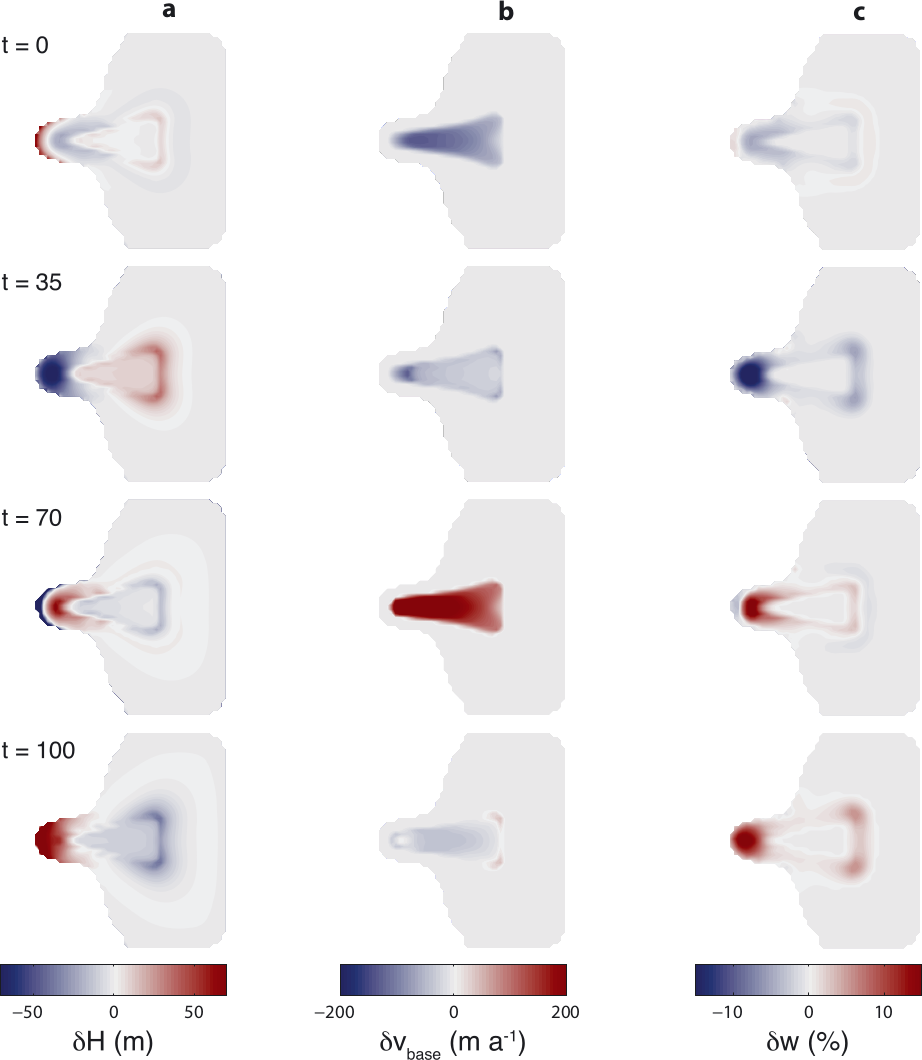
\includegraphics[width=0.8\textwidth]{figs/vanPeltOerlemans-fig4}

\medskip
\scriptsize (van Pelt \& Oerlemans, 2012, \emph{J.~Glaciol.})
\end{center}
\end{column}
\end{columns}
\end{frame}


\begin{frame}
  \frametitle{goal: improve PISM by adding mass-conserving subglacial hydrology}

subgoals:

\begin{enumerate}
  \item \scream{provide reasonable default behavior}
  \item \scream{introduce a minimum number of new tunable parameters}
    %\item[$\ast$]<2-4> \dots that does no harm
  \item \scream{provide a playground for testing basal sliding models}
\end{enumerate}

\end{frame}




\begin{frame}
  \frametitle{elements of subglacial hydrology}
  \framesubtitle{we can agree on these?}

\newcommand{\bq}{\mathbf{q}}

  \begin{itemize}
    \item \textbf{conservation of mass}:
    
    $$W_t + \nabla \cdot \bq = m / \rho_w$$

where $W=$ spatially-averaged thickness of water layer, $\bq=$ flux, $m=$ supply rate ($\text{kg}\,\text{m}^{-2}\,\text{s}^{-1}$)

    \begin{onlyenv}<1>\item \textbf{hydraulic potential}:
    
    $$\phi = p_w + \rho_w g b$$

where $\phi=$ hydraulic potential, $b=$ bedrock elevation
    \end{onlyenv}

    \begin{onlyenv}<2>\item \textbf{hydraulic potential} {\color{blue} for top of water sheet}:
    
    $$\phi = p_w + \rho_w g (b{\color{blue} + W})$$

where $\phi=$ hydraulic potential, $b=$ bedrock elevation
    \end{onlyenv}

    \item \textbf{some kind of Darcy flow}:
    
    $$\bq = - \frac{K W}{\rho_w g} \nabla \phi$$
    
    \scriptsize or \quad $\bq = - k W^\alpha |\nabla \phi|^{\beta - 2} \nabla \phi$ \quad etc.
    
\normalsize where $K=$ hydraulic conductivity (\emph{not} constant in general)
  \end{itemize}

\end{frame}


\begin{frame}
  \frametitle{elements of subglacial hydrology}
  \framesubtitle{whence pressure?}

  \begin{itemize}
    \item combine previous three equations to get one equation in two unknown fields: $W$ and $p_w$
    \item an equation is needed to determine the pressure $p_w$
    \item some alternatives:
      \begin{itemize}
      \item[$\ast$] creep dominates, zero effective pressure (e.g.~slow subglacial lake):
        $$p_w = \rho_i g H$$
      \item[$\ast$] generates porous medium equation (Flowers \& Clarke 2002):
        $$p_w = \rho_i g H \left(\frac{W}{W_{\text{crit}}}\right)^\gamma$$
        where $\gamma=7/2$ and $W_{\text{crit}}=0.1$ m, for example
      \end{itemize}
  \end{itemize}

\end{frame}


\begin{frame}
  \frametitle{elements of subglacial hydrology}
  \framesubtitle{whence pressure? (more alternatives)}

  \begin{itemize}
    \item another alternative:
      \begin{itemize}
      \item[$\ast$] physical models for opening and closure of a distributed system
        \begin{itemize}
        \item[$\circ$]  evolution equation for [$Y=$ average cavity depth] must be of the form
        $$Y_t = W_O - W_C$$
where $W_O$ is the total opening effect from a longish list of processes (wall melt, sliding, \dots) and $W_C$ is the total closing effect from a list of processes including creep (Hewitt, 2011)
        \item[$\circ$] indirectly this determines water pressure $p_w$
        \end{itemize}
      \item[$\ast$] but wait: there are channels, too! (R\"othlisberger)

\begin{center}
\medskip
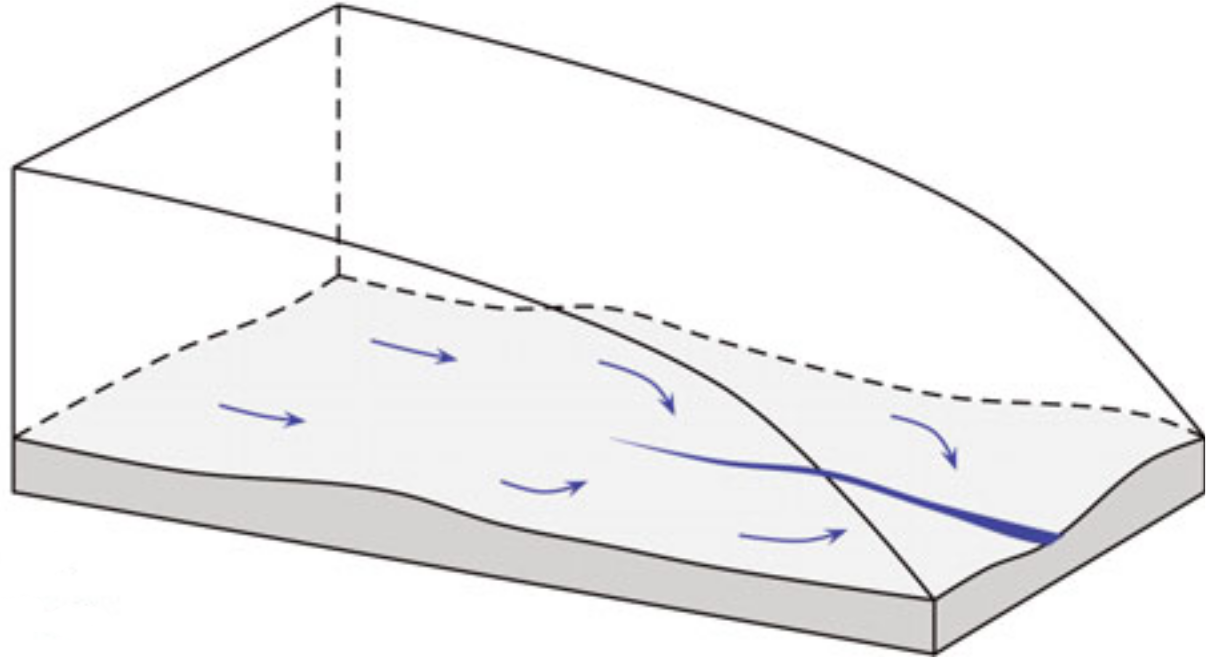
\includegraphics[width=0.4\textwidth]{figs/hewitt-cartoon} \tiny figure from (Hewitt, 2011)
\medskip
\end{center}
    \end{itemize}
  \end{itemize}
\end{frame}


\begin{frame}
  \frametitle{elements of subglacial hydrology}
  \framesubtitle{whence pressure? (yet more alternatives from Vancouver, B.C.~area)}

  \begin{itemize}
  \item  Schoof (2010): fixed-location network of channels
  \item Schoof and Hewitt and Werder (2012): elliptic variational inequality determines water pressure
  \end{itemize}

\end{frame}



\begin{frame}
  \frametitle{TMI}

  \begin{itemize}
  \item too much information!
  \item \dots and too many tunable parameters
    \begin{itemize}
    \item[$\ast$] even though I \emph{like} elliptic variational inequalities
    \end{itemize}
  \item yes, we hope to explore these alternatives in PISM
  \item but it has finally dawned on us:
  
  \begin{center}
  \emph{exploring processes through modeling is different from improving default behavior for ice sheet simulation}
  \end{center}
  \end{itemize}
\end{frame}


\begin{frame}
  \frametitle{back to something basic}

  \begin{itemize}
    \item recall the simple model where creep dominates:
    		$$p_w = \rho_i g H$$
    \item then hydraulic potential comes from three heights (underlined):
    \begin{align*}
      \phi &= \rho_i g H + \rho_w g (b+W) \\
           &= \rho_i g \underline{\phantom{|}h\phantom{|}} + (\rho_w - \rho_i) g \underline{\phantom{|}b\phantom{|}} + \rho_w g \underline{\phantom{|}W\phantom{|}}
    \end{align*}
    \item<2-3> combining all equations gives a simple equation for water thickness:
       $$\boxed{W_t + \nabla\cdot\left(\mathbf{v} W\right) = K \nabla \cdot(W \nabla W) + m / \rho_w}$$
      \begin{itemize}
      \vspace{-6mm}
      \item[$\ast$] where $\mathbf{v} = - K \left[r \nabla h + (1-r) \nabla b\right]$
      \item[$\ast$] \dots if $r = \rho_i/\rho_w$
      \item[$\ast$] it is an advection-diffusion equation
      \end{itemize}
    \item<3> \scriptsize generalization with one tunable parameter $0<s<1$: \quad $p_w = s\, \rho_i g H$
  \end{itemize}
\end{frame}


\begin{frame}
  \frametitle{time scales with the simple choice}

  \begin{itemize}
    \item FIXME: equation for $\mathbf{v}$: comment \& show results
  \end{itemize}

\end{frame}


\begin{frame}
  \frametitle{results from the simple choice}

  \begin{itemize}
    \item FIXME: show for EAIS
  \end{itemize}

\end{frame}


\begin{frame}
  \frametitle{a goal we can achieve with this model}
 
\begin{center}
  \scream{report the amount of subglacial water delivered at each outlet}
\end{center}
  
  \begin{itemize}
    \item we can do this for ice flow because we know which direction the ice flows
    \item we need a subglacial hydrology just to know which fjord gets the water
  \end{itemize}

\begin{columns}
\begin{column}{0.5\textwidth}
\begin{center}
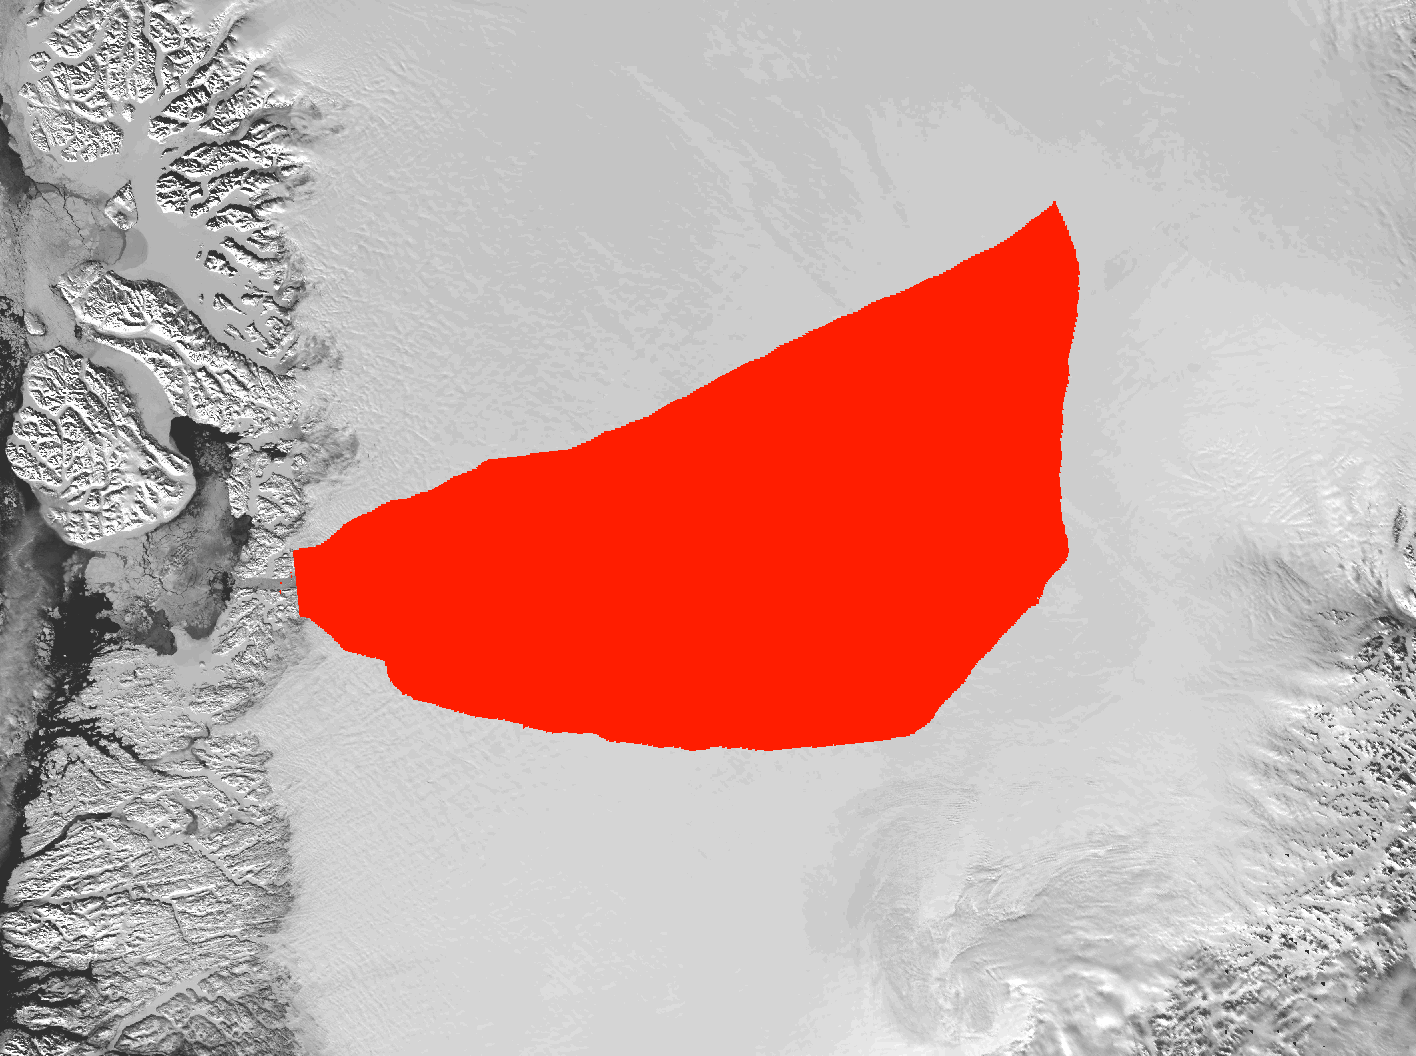
\includegraphics[width=0.7\textwidth]{figs/ftt-mask}
\end{center}
\end{column}
\begin{column}{0.5\textwidth}
\begin{center}
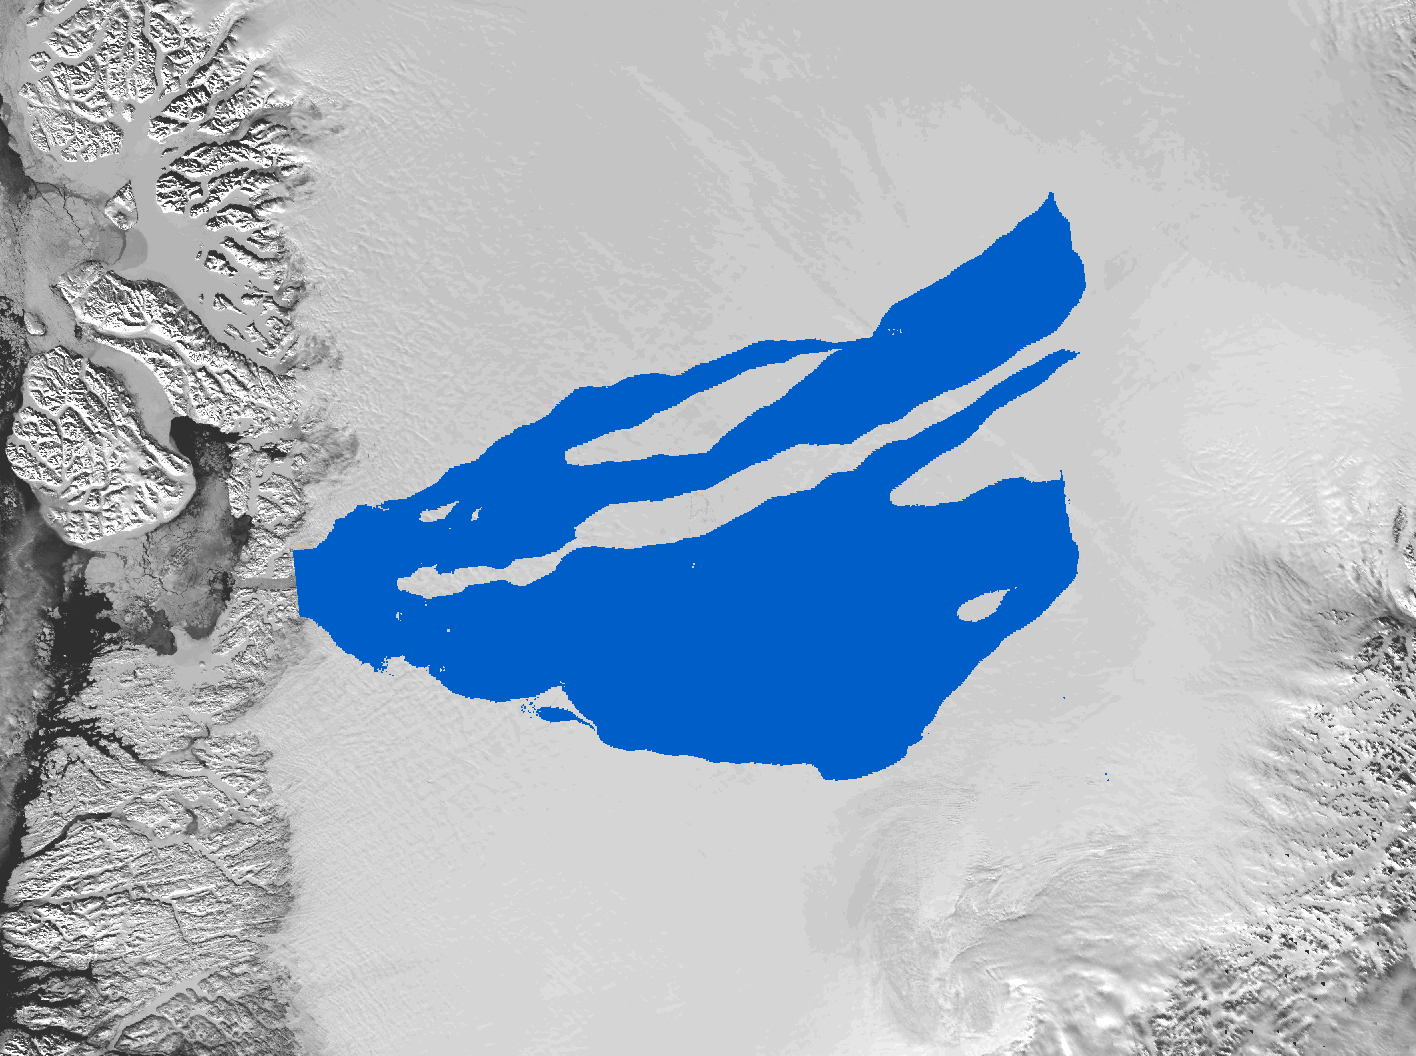
\includegraphics[width=0.7\textwidth]{figs/hydro-mask}
\end{center}
\end{column}
\end{columns}

\end{frame}


\setbeamertemplate{background canvas}
{
  \tikz{\node[inner sep=0pt,opacity=0.3] {\includegraphics[width=\paperwidth]{figs/crop-andy-66}};}
} 


\begin{frame}
  \frametitle{FIXME: summary}

\small
  \begin{itemize}
  \item channeling flow can only be implemented in a 2d framework when the position of the channels is predefined; this does not seem to be desirable in our approach
  \item main problem at the moment is the interaction/feedback of the water flux and the wall melt term in the opening/closure-equation. This interaction ultimately leads to concentrated water flow in infinitely narrow channels (larger water flux ->  larger channel -> lower pressure -> larger water flux)
  \item We leave out the wall melt term in the closure relation and hence only model linked-cavity flow (opening by cavitation balanced by creep closure). This model would be suitable for all regions of an ice sheet except for fast flowing outlet glaciers.
  \item Make the wall melt opening term in the opening/closure-relation a function of the water input rate rather than the water flux.
  \item \alert{great danger} in building a model whose parameters cannot be identified
  \end{itemize}
  
  \begin{center}
  \tiny Thanks for help with talk: Andy Aschwanden, Sarah Child, Brad Gooch.
  \end{center}
\end{frame}








\end{document}
